\documentclass{beamer}
\usepackage{graphicx}
\usepackage{amsmath}

\title{Scalable Overlay Operations over DCEL Polygon Layers}
\author{Andres Oswaldo Calderon Romero}
\institute{University of California, Riverside}
\date{November 2024}

\begin{document}

\begin{frame}
    \titlepage
\end{frame}

\begin{frame}
    \frametitle{Introduction}
    \begin{itemize}
        \item Spatial data structures, especially DCEL, are essential for various spatial applications.
        \item Doubly Connected Edge List (DCEL) helps manage topological information of edges, vertices, and faces.
        \item Overlay operations enable integration of different spatial data layers.
        \item This work addresses scalability challenges for overlay computations over DCEL layers.
    \end{itemize}
\end{frame}

\begin{frame}
    \frametitle{Motivation and Problem Statement}
    \begin{itemize}
        \item Large spatial datasets (e.g., US census tracts) make traditional DCEL overlay operations challenging.
        \item Need for scalable, distributed DCEL overlay solutions.
        \item Objectives:
        \begin{itemize}
            \item Efficient partitioning and merging for scalable DCEL overlays.
            \item Enable parallel overlay operations while maintaining data integrity.
        \end{itemize}
    \end{itemize}
\end{frame}

\begin{frame}
    \frametitle{Related Work}
    \begin{itemize}
        \item Historical use of DCEL in various applications (e.g., computational geometry, 3D graphics).
        \item Existing sequential algorithms for overlay operations: LEDA, CGAL.
        \item Need for scalable, parallel approaches in spatial data processing.
    \end{itemize}
\end{frame}

\begin{frame}
    \frametitle{DCEL Overview}
    \begin{itemize}
        \item DCEL consists of vertices, edges (half-edges), and faces.
        \item Each half-edge has references to twin, next, and previous edges.
        \item Allows efficient topological and geometric queries.
    \end{itemize}
    \begin{figure}
        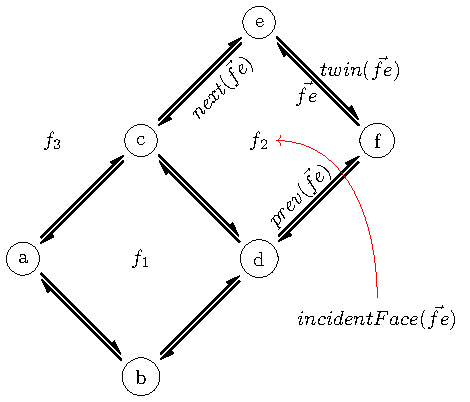
\includegraphics[width=0.5\textwidth]{chapterSDCEL/dcel_example/dcel_example} % Add your own diagram here
        \caption{DCEL Structure}
    \end{figure}
\end{frame}

\begin{frame}
    \frametitle{Scalable Overlay Construction}
    \begin{itemize}
        \item Partition Strategy: Quadtree-based partitioning to manage large datasets.
        \item Each cell in the quadtree can be processed independently.
        \item Local results merged to form global overlay.
    \end{itemize}
    \begin{figure}
        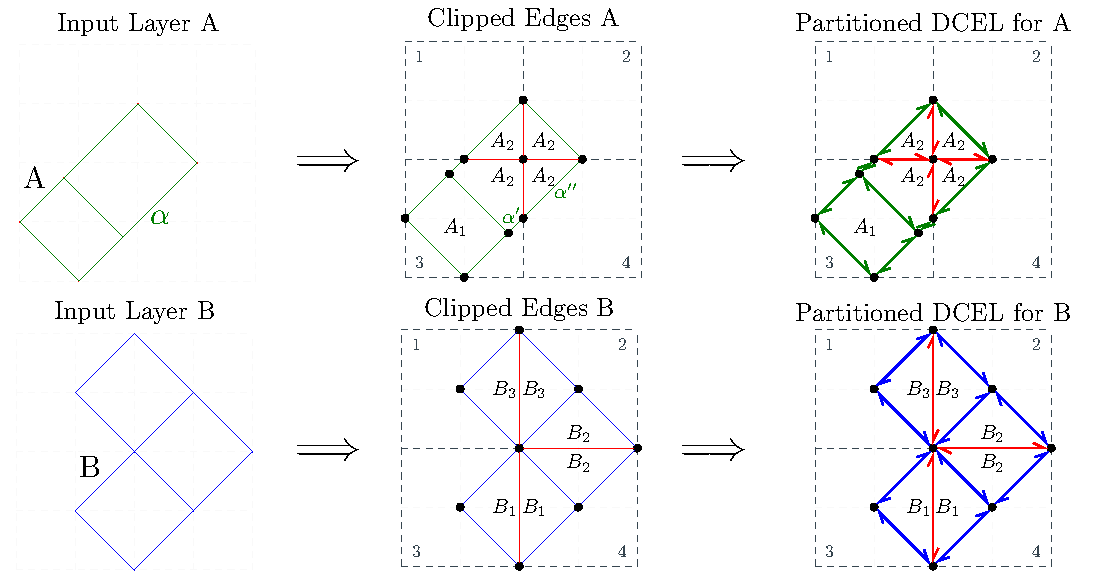
\includegraphics[width=0.6\textwidth]{chapterSDCEL/partition_schema/PolygonsParted} % Add partitioning figure here
        \caption{Partitioning Strategy for Overlay Computation}
    \end{figure}
\end{frame}

\begin{frame}
    \frametitle{Handling Orphan Cells and Holes}
    \begin{itemize}
        \item Problem: Holes or faces spanning multiple cells require special handling.
        \item Solution: Label propagation using quadtree structure.
        \item Recursive search for label consistency across partitions.
    \end{itemize}
\end{frame}

\begin{frame}
    \frametitle{Optimization Strategies}
    \begin{itemize}
        \item Optimization for Faces Spanning Multiple Cells
            \begin{itemize}
                \item Intermediate reduce phase to handle large number of faces.
                \item Spatial proximity property to minimize central node workload.
            \end{itemize}
        \item Optimization for Unbalanced Layers
            \begin{itemize}
                \item Focused scanning of dense layers to improve performance.
            \end{itemize}
    \end{itemize}
\end{frame}

\begin{frame}
    \frametitle{Experimental Evaluation}
    \begin{itemize}
        \item Datasets: MainUS, GADM, CCT
        \item Evaluation metrics: Runtime, scalability, efficiency.
        \item Comparison with baseline approaches like CGAL.
    \end{itemize}
\end{frame}

\begin{frame}
    \frametitle{Results and Observations}
    \begin{itemize}
        \item Partitioning improves overlay operation efficiency.
        \item Optimizations reduce computation time, especially in unbalanced datasets.
        \item Scalable solution performs significantly better on large datasets than sequential methods.
    \end{itemize}
\end{frame}

\begin{frame}
    \frametitle{Conclusions}
    \begin{itemize}
        \item Developed a scalable overlay computation for DCEL layers.
        \item Approach supports distributed, efficient DCEL operations.
        \item Future work: Further improvements in handling extremely dense data.
    \end{itemize}
\end{frame}

\end{document}
